\begin{figure}[h]
	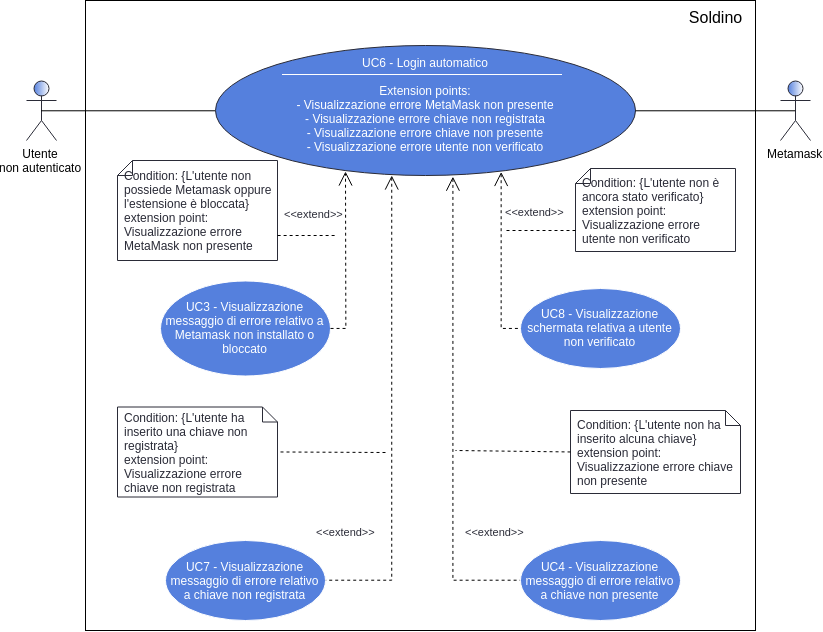
\includegraphics[width=12cm]{res/images/login.png} %da adattare in larghezza
	\centering
	\caption{Schema generale: login ed errori annessi}
	
\end{figure}
\subsubsection{UC6 - Login automatico}
\begin{itemize}
	\item \textbf{Attori Primari}:
	utente non autenticato;
	\item \textbf{Attori Secondari}:
	MetaMask\glo;
	\item \textbf{Descrizione}:
	in modo automatico, il sistema procede all'identificazione dell'utente;
	\item \textbf{Scenario principale}:
	l'utente non ancora autenticato richiede il login;
	\item \textbf{Estensioni}:
	\begin{itemize}
		\item \textbf{UC3}: se l'utente non dispone di MetaMask\glosp o ha disabilitato l'estensione, viene visualizzato un messaggio di errore a riguardo;
		\item \textbf{UC4}: se l'utente non possiede una chiave\glosp su MetaMask\glo, esso viene avvisato tramite l'apposito messaggio di errore;
		\item \textbf{UC7}: se l'utente tenta di accedere al sito tramite MetaMask\glosp senza aver mai provveduto a registrarsi, riceverà un messaggio di errore a riguardo;
		
		\item \textbf{UC8}: se l'utente si è registrato ma il suo account è stato disabilitato, riceverà un messaggio di errore a riguardo.
	\end{itemize}
	\item \textbf{Precondizione}:
	l'utente tenta di autenticarsi alla piattaforma;
	\item \textbf{Postcondizione}:
	l'utente si è autenticato con successo, ed è stato identificato dal sistema nel ruolo di cittadino, azienda o utente governativo. A seconda della tipologia di utente vengono rese disponili diverse pagine e funzionalità.
\end{itemize}
\subsubsection{UC7 - Visualizzazione messaggio di errore relativo a chiave non registrata}
\begin{itemize}
	\item \textbf{Attori Primari}:
	utente non autenticato;
	\item \textbf{Descrizione}:
	l'utente visualizza un messaggio di errore dovuto al fatto che ha tentato il login senza essersi registrato in precedenza;
	\item \textbf{Scenario principale}:
	l'utente tenta di eseguire la procedura di login alla piattaforma senza essere registrato;
	\item \textbf{Precondizione}:
	l'utente tenta di autenticarsi nella piattaforma;
	\item \textbf{Postcondizione}: viene visualizzato un messaggio d'errore per informare l'utente del fatto che è necessario registrarsi alla piattaforma prima di poter poi effettuare la procedura di login.
\end{itemize}
\subsubsection{UC8 - Visualizzazione schermata relativa a utente non abilitato}
\begin{itemize}
	\item \textbf{Attori Primari}: utente non autenticato;
	\item \textbf{Descrizione}:
	l'utente tenta di autenticarsi alla piattaforma, tuttavia, a causa della disabilitazione del suo account, il login viene interrotto e l'utente visualizza il messaggio personalizzato lasciato dal governo che illustra la causa della disabilitazione dell'account;
	\item \textbf{Scenario principale}:
	l'utente non autenticato con account disabilitato tenta di autenticarsi. La procedura di autenticazione viene bloccata a causa dello stato dell'account;
	\item \textbf{Precondizione}:
	un utente non autenticato, registrato alla piattaforma e con account disabilitato tenta di effettuare il login automatico;
	\item \textbf{Postcondizione}:  viene visualizzato un messaggio d'errore per informare l'utente del fatto che il proprio account è stato disabilitato dal governo. Se quest'ultimo, durante la procedura di disabilitazione, ha inserito un messaggio contenente la causa di tale azione, allora tale messaggio viene visualizzato.
\end{itemize}
\begin{figure}[h]
	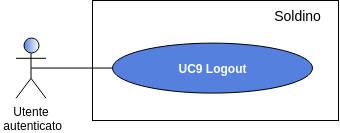
\includegraphics[width=6cm]{res/images/UC9-Logout.png} %da adattare in larghezza
	\centering
	\caption{UC9 - Logout}
	
\end{figure}
\subsubsection{UC9 - Logout}
\begin{itemize}
	\item \textbf{Attori Primari}:
	utente autenticato;
	\item \textbf{Attori Secondari}:
	MetaMask\glo;
	\item \textbf{Descrizione}: l'utente richiede il logout dalla piattaforma web. Vengono visualizzate le informazioni necessarie per procedere alla procedura di logout, che deve essere effettuata attraverso l'utilizzo del plug-in MetaMask\glo;
	\item \textbf{Scenario principale}: l'utente è autenticato dal sito e richiede di effettuare il logout, premendo sull'apposito pulsante;
	\item \textbf{Precondizione}: l'utente ha effettuato il login alla piattaforma web e richiede di essere disconnesso dal sito;
	\item \textbf{Postcondizione}: vengono visualizzate le istruzioni necessarie per eseguire il logout tramite MetaMask\glo. 
\end{itemize}

